\section{Resultados Obtenidos}

\begin{frame}{Resultados Obtenidos (1/7)}
\framesubtitle{Metodolog\'ia}

\framesubtitle{An\'alisis de Datos}
\vspace{-0.5em}
\begin{table}[H]
\centering
\footnotesize
\begin{tabular}{|p{1.2cm}|p{5.5cm}|p{2cm}}
\hhline{--~}
M\'etrica  &   Descripci\'on & \\
\hhline{--~}
$M$ &       12,75 palabras & \rdelim\}{1}{2cm}[Memoria del Usuario] \\
$A$  &      83,70 \% & \rdelim\}{2}{2cm}[\parbox{3cm-\tabcolsep-\widthof{$\Bigg]$}}{Correctitud de la Aplicaci\'on}] \\
$E_1$ &     16,30 \%  \\
$E_2$ &     5,91 \% &  \rdelim\}{2}{2cm}[Error Humano] \\
$E_3$ &    11,83 errores  \\
$T_{1+2}$ & 13,83 minutos  & \rdelim\}{4}{2cm}[Eficiencia] \\
$T_{3+4}$ & 18,35 minutos \\
$C$ &       87,5 \%  \\
$U$ &       40.67 comandos \\
\cline{1-2} 
\end{tabular}
\end{table}
\end{frame}

\begin{frame}{Resulados Obtenidos (2/7)}
\framesubtitle{Correlaci\'on}

\begin{itemize}
    \only<1-1>{\item $A$ y $E_2$, 0,51
    \item $A$ y $E_3$, 0,69}
    
    \only<2-2>{\item $U$ y $E_2$, 0,35
    \item $U$ y $E_3$, 0,52
    \item $U$ y $A$, 0,53}
   
    \only<3-3>{\item $M$ y $E_2$, -0,38
    \item $M$ y $T_{1+2}$, -0,31
    \item $M$ y $T_{3+4}$, -0,42}
\end{itemize}
\end{frame}

\begin{frame}{Resulados Obtenidos (3/7)}
\framesubtitle{Correlaci\'on}

\begin{itemize}
    \uncover<+->{\item $A$ y $C$, 0,50}

    \uncover<+->{\item $E_2$ y $T_{1+2}$, 0,40 
    \item $E_3$ y $T_{1+2}$, 0,57
    \item $E_3$ y $T_{3+4}$, 0,37}
\end{itemize}

%\begin{table}[H ] 
%\centering
%\footnotesize
%\begin{tabular}{|p{0.5cm}|p{0.75cm}|p{0.7cm}|p{0.75cm}|p{0.75cm}|p{0.75cm}|p{0.75cm}|p{0.75cm}|p{0.7cm}|p{0.75cm}|}
%\hline
%& $M$ &  $A$  &   $E_1$ &  $E_2$  &  $T_{1+2}$  & $T_{3+4}$     & $E_3$ & $C$ & $U$ \\
%\hline
%$M$       &  1     &  0,22  & -0,22  & \textbf{-0,38}  &  \textbf{-0,31}  &  \textbf{-0,42}  &  -0,29 & -0,08    &  -0,23 \\
%$A$       &  0,22  &  1  &  -1  &  \textbf{0,51}  &  0,14  &  -0,09  &  \textbf{0,69}  &  \textbf{0,5}           &  \textbf{0,53} \\
%$E_1$     &  -0,22 &  -1  &  1  &  \textbf{-0,51}  &  -0,14  &  0,09  &  \textbf{-0,69}  &  \textbf{-0,5}        &  \textbf{-0,53} \\
%$E_2$     &  \textbf{-0,38} &  \textbf{0,51}  &  \textbf{-0,51}  &  1  &  \textbf{0,4}  &  0,23  &  \textbf{0,71}  &  0,29         &  0,35  \\
%$T_{1+2}$ &  \textbf{-0,31} &  0,14  &  -0,14  &  \textbf{0,4}  &  1  &  \textbf{0,87}  &  \textbf{0,57}  &  -0,04        &  0,25 \\
%$T_{3+4}$ &  \textbf{-0,42} &  -0,09  &  0,09  &  0,23  &  \textbf{0,87}  &  1  &  0,37  &  -0,16       &  0,2 \\
%$E_3$     &  -0,29 &  \textbf{0,69}  &  \textbf{-0,69}  &  \textbf{0,71}  &  \textbf{0,57}  &  \textbf{0,37}  &  1  &  0,28        &  \textbf{0,52} \\
%$C$       &  -0,08 &  \textbf{0,5}  &  \textbf{-0,5}  &  0,29  &  -0,04  &  -0,16  &  0,28  &  1        &  0,13 \\
%$U$       &  -0,23 &  \textbf{0,53}  &  \textbf{-0,53}  &  \textbf{0,35}  &  0,25  &  0,2  &  \textbf{0,52}  &  0,13      &  1 \\
%\hline
%\end{tabular}
%\caption{Coeficientes de correlaci\'on para las m\'etricas consideradas.}
%\label{sec:tabla-correlacion}
%\end{table}

\end{frame}

\begin{frame}{Resultados Obtenidos (4/7)}
\framesubtitle{An\'alisis del Error Humano}

\uncover<+->{\begin{table}[H]
\centering
\footnotesize
\begin{tabular}{|p{1.2cm}|p{1.0cm}|p{1.0cm}|p{1.0cm}|p{1.0cm}|p{1.0cm}|}
\hline
    Longitud & 2 & 3 & 4 & 5 & 6  \\
    \hline 
    Promedio & 6,96 & 5,68 & 7,46 & 14,81 & 42,11 \\
\hline
\end{tabular}
\caption{Tasa de error humano por longitud del comando.}
\label{sec:error-longitud}
\end{table}}

\uncover<+->{\begin{table}[H]
\centering
\footnotesize
\begin{tabular}{|p{1.6cm}|p{1.6cm}|p{1.6cm}|p{1.6cm}|}
\hline
    Contexto & General & Pista & Comp\'as \\
\hline
Promedio & 13,25 & 3,57 & 5,16 \\
\hline
\end{tabular}
\caption{Tasa de error humano por nivel contextual del comando.}
\label{sec:error-contexto}
\end{table}}


\uncover<+->{\begin{table}[H]
\centering
\footnotesize
\begin{tabular}{|l|p{3cm}|}
\hline
Comando & Tasa de Error \\
\hline
crear nueva partitura & 18,38 \\
duplicar pista uno en pista dos & 17,5 \\
duplicar pista uno en pista tres & 16,67 \\
duplicar pista tres en pista cuatro & 13,25 \\
comp\'as cuatro & 13,19 \\
\hline
\end{tabular}
\caption{Lista de comandos con mayor tasa de error humano promedio.}
\label{sec:tabla-lista-comandos-error}
\end{table}}


\end{frame}


\begin{frame}{Resultados Obtenidos (5/7)}
\framesubtitle{An\'alisis del Error Humano}

\begin{columns}
\column{0.3\linewidth}
\centering
\begin{table}
\tiny
\begin{tabular}{|c|c|}
\hline
    Etapa & \% de la Tasa \\ & de Error Total \\
    \hline
0-10  &  11,62 \\
10-20 &  13.49 \\
20-30 &  12,29 \\
30-40 &  17,78 \\
40-50 &  6,85 \\
50-60 &  3,75 \\
60-70 &  9,92 \\
70-80 &  2,76 \\
80-90 &  12,12 \\
90-100 & 9,42 \\
    \hline
\end{tabular}
\caption{Distribuci\'on del error humano por etapas de la sesi\'on.}
\label{sec:error-tiempo}
\end{table}
\column{0.7\linewidth}
\begin{figure}
\centering
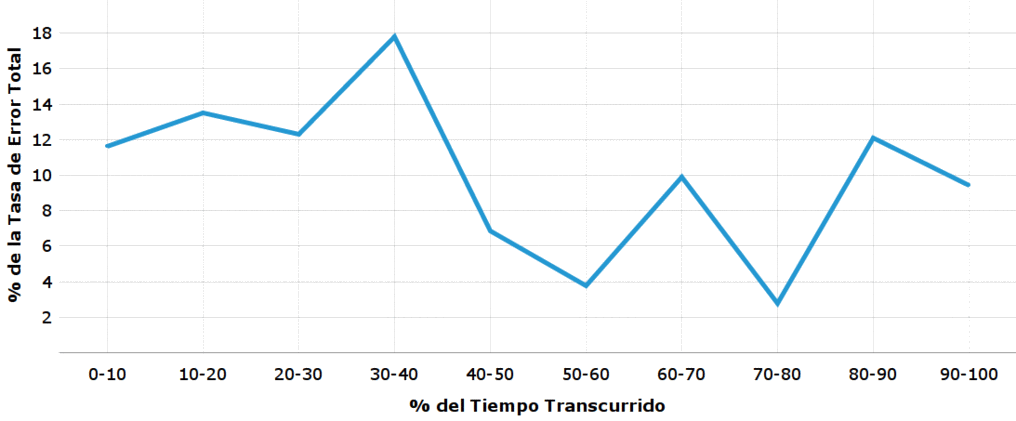
\includegraphics[width=1\linewidth]{./graphics/error_tiempo.png}
\caption{Distribuci\'on del error humano por etapas de la sesi\'on.}
\label{figure:gerror-tiempo}
\end{figure}
\end{columns}

\end{frame}

\begin{frame}{Resultados Obtenidos (6/7)}
\framesubtitle{Encuesta}
\begin{columns}
\column{0.35\linewidth}
\begin{table}[H] 
\centering
\tiny
\begin{tabular}{|r|r|r|r|r|}
\hline
            & Promedio \\
\hline
Vocabulario    & 6.17 \\
Comandos    & 6.58 \\
Entrenamiento  & 6.25 \\
Interfaz por Voz & 5.83 \\
\hline
\end{tabular}
\caption{Resumen de la encuesta realizada.}
\label{sec:tabla-encuesta}
\end{table} 
\column{0.65\linewidth}
\begin{figure}[ht]
\centering
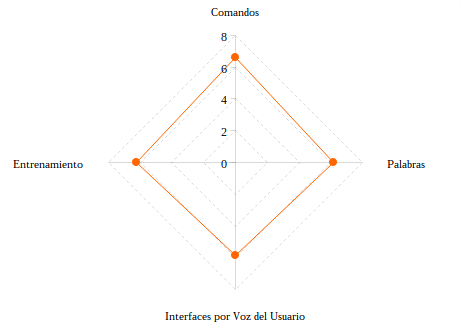
\includegraphics[width=1\linewidth]{./graphics/kiviat0.png}
\caption{Gr\'afico radial resumen de la encuesta realizada.}
\label{figure:kiviat-encuesta1}
\end{figure}
\end{columns}
\end{frame}

\begin{frame}{Resultados Obtenidos (7/7)}
\framesubtitle{Encuesta}
\begin{columns}
\column{0.35\linewidth}
\begin{table}[H] 
\centering
\tiny
\begin{tabular}{|r|r|r|r|r|}
\hline
            & Promedio \\
\hline
Vocabulario    & 0.45 \\
Comandos    & 0.86 \\
Entrenamiento  & 0.55 \\
Interfaz por Voz & 0.5 \\
\hline
\end{tabular}
\caption{Resumen de la encuesta realizada. Valores reescalados.}
\label{sec:tabla-encuesta-normalizada}
\end{table}
\column{0.65\linewidth}
\begin{figure}[ht]
\centering
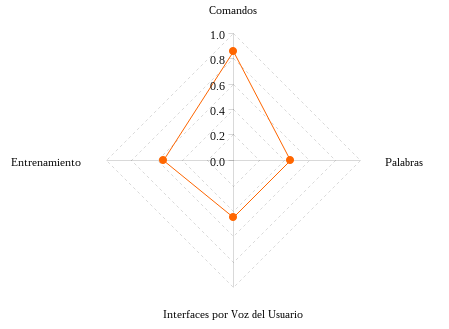
\includegraphics[width=1\linewidth]{./graphics/kiviat.png}
\caption{Gr\'afico radial resumen de la encuesta realizada. Valores reescalados.}
\label{figure:kiviat-encuesta2}
\end{figure}
\end{columns}
\end{frame}